\subsection{Desarrollo}

\subsubsection{Encontrando matriz banda p,q}

Como dice el enunciado, cada una de las $2n$ juntas aporta 2 nuevas ecuaciones. El sistema lineal resultante tiene por lo tanto $4n$ ecuaciones con $4n$ incógnitas.
Intuitivamente lo que buscamos es que los números identificadores de las variables que actúan sobre una misma junta sean cercanos entre sí (Eso implica una buena numeración sobre los links de la estructura,
que respresentarán las variables).
Al mismo tiempo queremos que las juntas en donde interviene un determinado link no queden lejos entre sí (Eso implica una buena numeración sobre las juntas de la estructura, que respresentarán las filas).
En primer lugar, para encontrar la matriz banda $B_{p,q}$ dibujamos un puente Pratt Truss de 8 secciones y miramos fijamente la estructura tratando de realizar deducciones al respecto.

Si miramos a las juntas de a pares verticales: \{c1,c2\}, \{c3,c4\}, \ldots podemos advertir que por cada nuevo par se presentan 4 nuevas fuerzas. A su vez, cada una de las juntas tiene asociada 2 ecuaciones
del sistema (Uno para las fuerzas horizontales y otro para las verticales). Entonces podemos pensar que se introducen 4 nuevas variables cada 4 ecuaciones (1 por ecuación). Por lo tanto, es razonable pensar
que con la numeración correcta podemos llegar a obtener una matriz banda $B_{p,q}$, ya que los coeficientes distintos de cero se concentrarían alrededor de la diagonal. Además, un determinado link solo actúa 
sobre 2 juntas. Indudablemente debemos aprovechar este hecho para establecer el valor $p$ de nuestra matriz. Una numeración razonable consiste en aplicarle (tanto a los links como a las juntas) valores en
forma creciente de izquierda a derecha, y de abajo hacia arriba, tal como está representado en el siguiente diagrama:

\begin{figure}[!h]
	\begin{center}
		  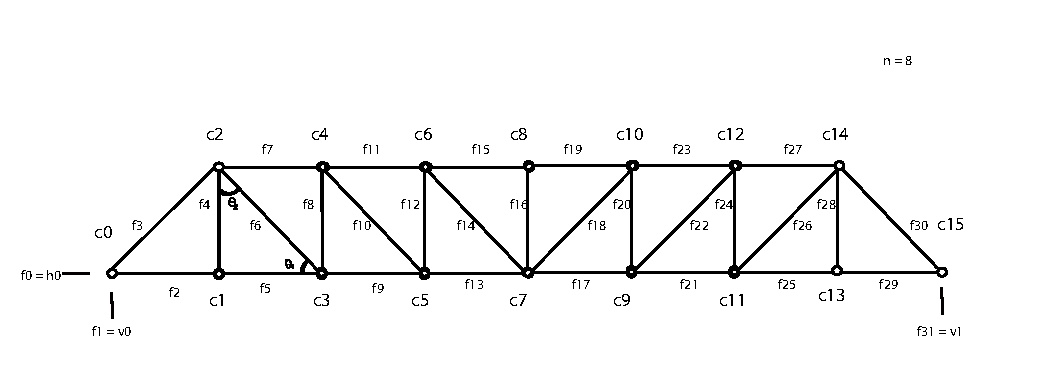
\includegraphics[keepaspectratio]{Imagenes/im_1.pdf}
		  \caption{Numeración para puente de 8 secciones}
		  \label{fig:contra1}
	\end{center}
\end{figure}
\FloatBarrier



\begin{figure}[!h]
	\begin{center}
		  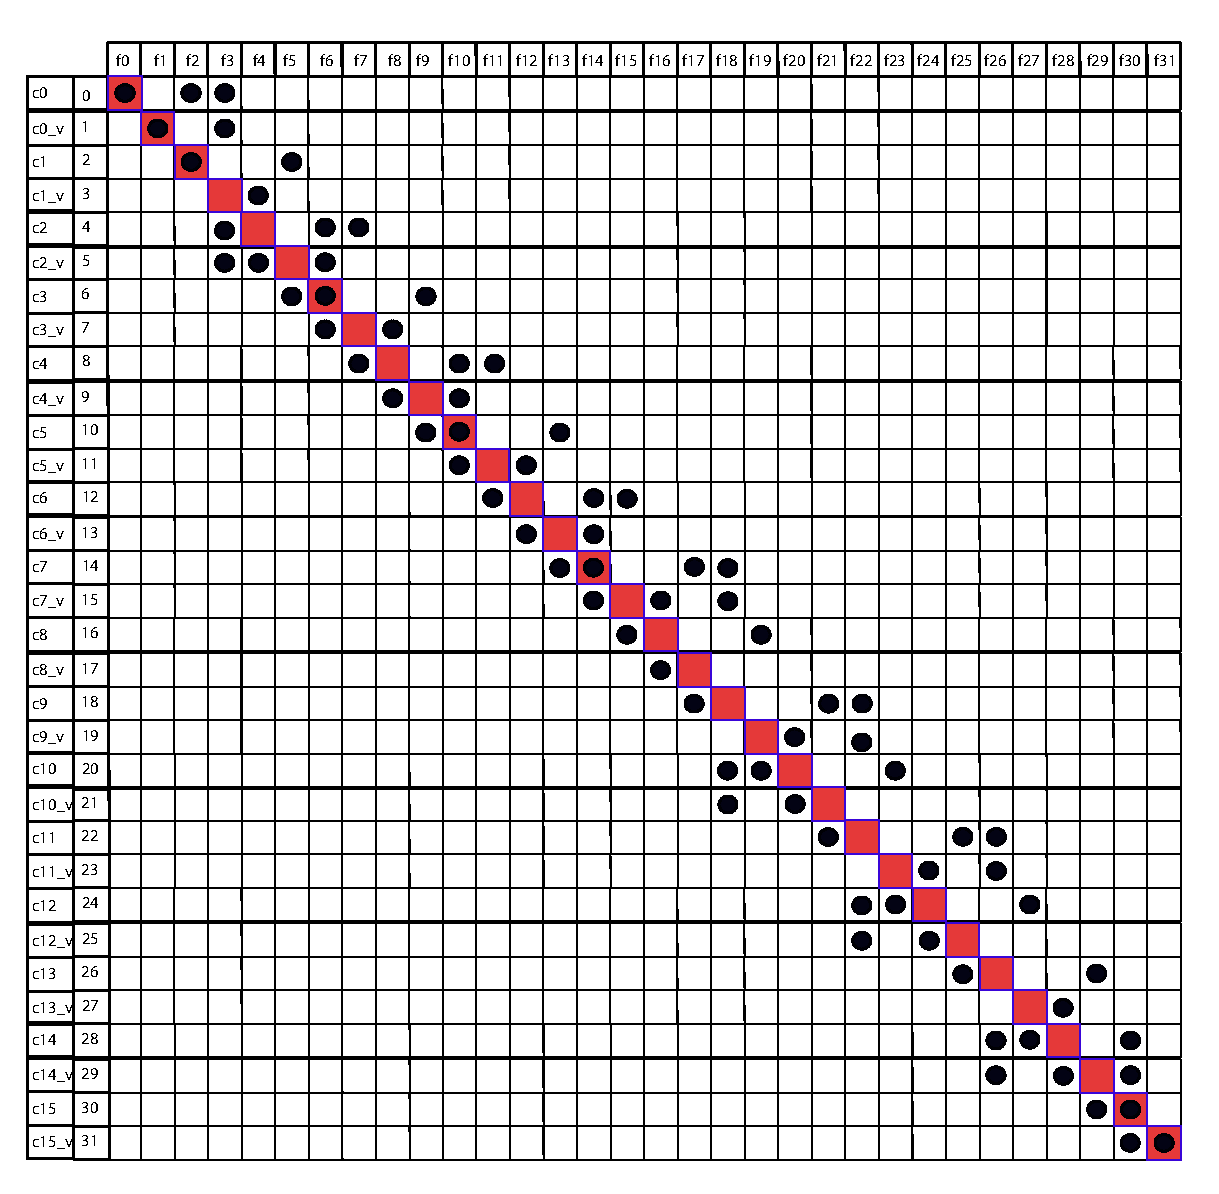
\includegraphics[scale=0.5]{Imagenes/im_2.pdf}
		  \caption{Esquema de matriz a partir del sistema de ecuaciones}
		  \label{fig:contra1}
	\end{center}
\end{figure}
\FloatBarrier